\documentclass[12pt,letterpaper]{article}

%%%%%%%%%%%%%%%%%%%%%%%%%
% Package configuration %
%%%%%%%%%%%%%%%%%%%%%%%%%

% Page margin
\usepackage[margin=1in]{geometry}

% Support for bold small cap font
\usepackage[tuenc]{fontspec}
\setmainfont[
    Path=./fonts/,
    Extension=.otf,
    BoldFont=cmu-serif-bold,
    BoldItalicFont=cmu-serif-bold-italic,
    ItalicFont=cmu-serif-italic,
]{cmu-serif}

% Better typesetting quality
\usepackage{microtype}

% Make letter spacing work for both XeLaTeX and LuaLaTeX
\usepackage{ifluatex}
\ifluatex
    \newcommand{\LSSTYLE}{\lsstyle}
\else
    \newcommand{\LSSTYLE}{\addfontfeatures{LetterSpace=12}}
\fi

% Math
\usepackage{amsmath}
\renewcommand{\vec}[1]{\mathbf{#1}}  % Bold as vector

% SI units
\usepackage{siunitx}

% Figure
\usepackage{float,graphicx}

% Redefine section, subsection styles
\usepackage[compact,center,explicit]{titlesec}
\usepackage{textcase}
\titleformat{\section}{\LSSTYLE\normalsize\scshape\filcenter}
    {\thesection}{1em}{\MakeTextUppercase{#1}}
\titleformat{\subsection}{\small\bfseries\filcenter}
    {\thesubsection}{1em}{#1}

% PRL-style horizontal rule
\usepackage{amssymb}
\newcommand{\PRLrule}{
    \bigskip
    \noindent\makebox[\linewidth]{
        \resizebox{0.3333\linewidth}{1pt}{$\blacklozenge$}
    }
    \bigskip
}

% Bold math in section title
\makeatletter
\g@addto@macro\bfseries{\boldmath}
\makeatother

% Set up author affiliation
\usepackage[affil-it]{authblk}

% Set up link, with (hopefully) math symbol support
\usepackage[pdfencoding=auto,psdextra]{hyperref}
\hypersetup{colorlinks,breaklinks,citecolor=blue}
\usepackage{cleveref}

% Set up biblatex database
\usepackage[
    %style=phys,
    giveninits=true,
    %backref=true,
    natbib=true,
    backend=biber,
    doi=true,
    % Sort by the order of citation
    sorting=none,
    % This options ensures that no automatic et al. is generated
    %maxbibnames=99,
    % This option must be enabled with 'babel' package
    useprefix=false
]{biblatex}
\addbibresource{umd_phd_candidacy_paper.bib}


%%%%%%%%%%%%%%%%%
% User settings %
%%%%%%%%%%%%%%%%%

% User-defined variables
\def\BaBar/{\textsc{BaBar}}
\def\Y4S/{\ensuremath{\Upsilon(\text{4S})}}
\def\RD/{\ensuremath{\mathcal{R}(D)}}
\def\RDst/{\ensuremath{\mathcal{R}(D^{*})}}
\def\RDDst/{\ensuremath{\mathcal{R}(D^{(*)})}}

% Title info
\title{Review on testing lepton flavor universality in semileptonic channels}
\author{Yipeng Sun}
\affil{Department of Physics, University of Maryland}
\date{\today}


%%%%%%%%%%%
% Content %
%%%%%%%%%%%

\begin{document}
\maketitle

\begin{abstract}
    What is LFUV? (FU physics, FUV physics)
    Why semileptonic decays (good thing about form factor)?
    A historical review, starting from 2012 BaBar;
    Talk about Phoebe's run 1 analyses.
    Talk about what we are doing.
    Talk about expected improvements and drawbacks of our upcoming analysis compared
    to run 1.
\end{abstract}


\section{Introduction}
The Standard Model (SM) has been very successful in describing the interactions
between elementary particles, such as quarks and leptons.
The theory has been tested experimentally to high precision.
However, there are phenomena that cannot be explained by the SM, such as
matter-antimatter asymmetry, hinting for some New Physics (NP) beyond the SM.
One way to search for NP is to measuring the decay rates of certain processes
very precisely;
rates that differ from the SM predictions may provide constraints on NP.

Though experimental discovery, it has been established that leptons have three
flavors:
Charged leptons, namely electron $e$, muon $\mu$, and tauon $\tau$;
their corresponding charge-neutral neutrinos: $\nu_e$, $\nu_\mu$ and $\nu_\tau$.
SM mandates that all three flavors of lepton participate in eletroweak
interaction with the same strength, except for the Higgs mechanism through which
they acquire their mass.
This is known as lepton flavor universality (LFU).

The LFU has been tested in many precision measurements, such as the decay rate
of $K^- \rightarrow e^- \nu_e$ versus $K^- \rightarrow \mu^- \nu_\mu$\footnote{
    Unless specified, charge conjugation is assumed.
}.
So far, no definite violation has been detected.
In this paper, we focus on the semileptonic decay channels of $B$ mesons, such
as $B^- \rightarrow D^{(*)} \l^- \overline{\nu}_l$:
Currently, the world average of the combined decay rate ratios $\RD/$ and
$\RDst/$, defined as\footnote{
    $\mathcal{B}$ denotes branching fraction.
}:
\begin{equation*}
    \RDDst/ \equiv \frac{
        \mathcal{B}\left(
            B^{0,-} \rightarrow D^{+,0(*)} \tau^- \overline{\nu}_\tau
        \right)
    }{
        \mathcal{B}\left(
            B^{0,-} \rightarrow D^{+,0(*)} \mu^- \overline{\nu}_\mu
        \right)
    }
\end{equation*}
has a $3.08\sigma$ deviation from the SM prediction, pointing to a possible
lepton flavor universality violation (LFUV);
many collaborations are working on more precise measurements to provide a
definite answer.

In the rest of the paper, we begin with a theoretical review on
why SM manifests LFU; possible extensions to SM, such as 2-Higgs doublet model
(2HDM), to permit LFUV; and advantages of using semileptonic channels for this
type of measurements.
We then review and compare colliders, such as $e^- e^+$ and hadron collider, and
detectors used in the testing of LFU.
After that, we will review previous experimental results.
Finally, we provide an overlook on updating $\RDDst/$ measurement with LHCb Run
2 data.


\section{Theory}
Leptons participate in electroweak interaction only;
the interaction can be described by a Lagrangian of the following form:
$\Lden{ew} = \Lden{gauge} + \Lden{f} + \Lden{\phi} + \Lden{Yuk}$.
The fermion part of \Lden{ew} reads \cite{Langacker:2010zza}:
\begin{align}
    \Lden{f} = \sum_{l = 1}^F \Big(
        & \bar{\spin{q}}^0_{lL} i \fsl{D} \spin{q}^0_{lL} +
          \bar{\spin{l}}^0_{lL} i \fsl{D} \spin{l}^0_{lL} + \nonumber \\
        & \bar{u}^0_{lR} i \fsl{D} u^0_{lR} +
          \bar{d}^0_{lR} i \fsl{D} d^0_{lR} +
          \bar{e}^0_{lR} i \fsl{D} e^0_{lR} +
          \bar{\nu}^0_{lR} i \fsl{D} \nu^0_{lR}
    \Big)
\end{align}
where the number $F$, empirically 3, of fermion flavors is summed over, and
$L,R$ denote $SU(2)_L$ doublet\footnote{
    The left-handed lepton doublet is defined as:
    $\spin{l}^0_{lL} = \begin{pmatrix} \nu_l \\ l \end{pmatrix}$,
    where $l$ denotes lepton flavor.
}
and singlet in each flavor generation.
From the Lagrangian we see that the interactions between fermions and gauge
bosons (the interactions are embedded in the \fsl{D} operator) is independent
of their flavor.
But this is only an incomplete picture:
Fermions acquire their mass through their interaction with the Higgs bosons,
which is omitted above.

No mass term of the form $m \overline{\Psi} \Psi$ is permitted, since it would
spoil $SU(2)$ symmetry of the Lagrangian\footnote{
    To be precise, \Lden{ew} is locally invariant under the transformations in
    $SU(2)_L \otimes U(1)$ group.
}.
Instead, we add a doublet scalar field $\Phi$ interacting on both gauge bosons
and fermions.
After spontaneous symmetry breaking of the vacuum state, the Lagrangian remains
unbroken, and the new terms in the Lagrangian are interpreted as mass terms.
We inspect the mass terms for the leptons \cite{Langacker:2010zza}\footnote{
    The notation has been simplified.
}:
\begin{equation}
    m_l \equiv \Gamma_l \frac{\nu}{\sqrt{2}}
\end{equation}
with $\nu$ interpreted as vacuum expectation value of $\Phi$.
This shows that leptons coupling stronger to the $\Phi$ (Higgs) field will be
more massive.

This completes the picture.
Now we see that SM demands LFU, except for the Higgs coupling.


\subsection{Advantages of semileptonic channel decays}

\subsection{Higgs mechanism}

\subsection{2-Higgs doublet models (2HDM)}
% type-II model claimed to be excluded; type-III (very similar to type-II) still
% alive.

\subsection{Leptoquark models}


\section{Review of colliders/detectors used in testing LFU}
The main reason is:
% Initially B factories are meant for CP violation detection.
Initially, detectors of $B$ factories, such as \BaBar/ at PEP-II, were
primarily constructed to for precision measurements on CP violation of $B^0$,
for SM predicts ``large, calculable'' CP violation in the decay of these mesons
\cite{Luth:1994}.
But these detectors proved to be advantageous in the testing of LFU:
These measurements have very similar requirements on the
detector \cite{Boutigny:1995ib}.
Thus, testing of LFU is often part of the secondary goals of these
experiments \cite{Luth:1994}.

In this section, I will review \BaBar/ detector at the PEP-II collider, and LHCb
at the Large Hadron Collider (LHC)---both have conducted various tests on LFU.
These detectors/colliders are representative of the detectors for
electron-position colliders and hadron colliders.

% Talk about PEP-II and its asymmetrical beam energies
PEP-II is an asymmetrical $e^- e^+$ collider at SLAC.
In PEP-II, $B$ mesons are produced primarily in the following process:
$e^- e^+ \rightarrow \Y4S/ \rightarrow B \bar{B}$, with
$e^-$ and $e^+$ beams tuned at different energies,
such that the invariant mass is at the \Y4S/ resonance (\SI{10.58}{GeV}),
and the momentum of the \Y4S/ in the lab frame
non-zero \cite{Harrison:1998yr}.

Producing at \Y4S/ peak eliminates almost all fragmentation products, reducing
combinatorial background.
Also, since the momenta of $e^- e^+$ is known, with the reconstruction of the
momentum of one $B$ meson ($B_{tag}$), the rest frame of the other $B$
($B_{sig}$) can be calculated as
\begin{equation}
    p_{B_{sig}} = p_{e^-e^+} - p_{B_{tag}}.
\end{equation}
Later we will see that this makes identifying events that have more than one
missing particle easier.

% Talk about subdetectors
\BaBar/ is a barrel detector (shown in \autoref{fig:babar_detector_view})
that consists of five subdetectors.
From inside out:
Silicon Vertex Tracker (SVT) and Drift Chamber (DCH), which measure the momenta
and angles of charged particles.
Detector of Internally Reflected Cerenkov radiation (DIRC), together with SVT
and DCH, identifies charged particles of different masses by Cerenkov
ring-imaging and ionization energy loss of these particles.
Caesium Iodide Electromagnetic Calorimeter (EMC), which measures energy and
position of electromagnetic showers generated by electrons and photons.
A superconducting solenoid with a \SI{1.5}{T} magnetic field surrounding the
EMC, together with Instrumented Flux Return (IFR), is used to identify muons and
some neutral hadrons \cite{Lees:2013uzd}.

\begin{figure}[ht]
    \centering
    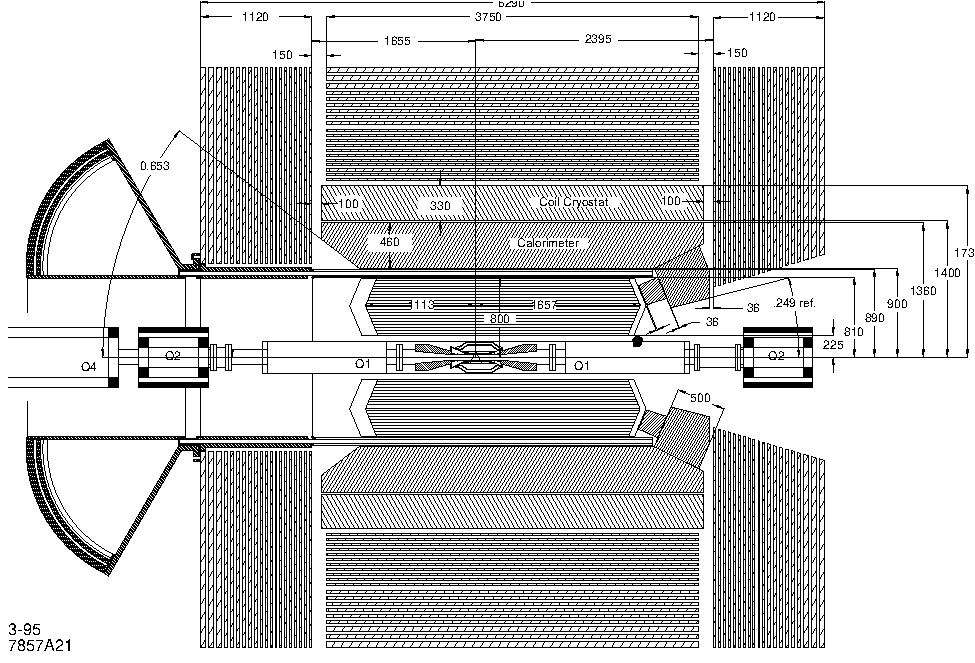
\includegraphics[width=0.7\textwidth]{figs/babar_detector_view.pdf}
    \caption{
        View of the \BaBar/ detector.
        Extracted from \cite{Boutigny:1995ib}.
    }
    \label{fig:babar_detector_view}
\end{figure}

% Talk about BaBar being 4 pi
In $e^- e^+$ detectors, $b \bar{b}$ is produced at all solid angles with
non-negligible probability \cite{Boutigny:1995ib,McGregor:2008ek}, thus the
detector needs to cover almost all solid angles (a $4\pi$ detector).
Indeed, \BaBar/ has tracking coverage of 0.92, namely 92\% of the $4\pi$ solid
angle.

% Talk about tracking and calorimeters
$B$ physics requires excellent vertex resolution and tracking, because the two
$B$ mesons produced by \Y4S/ must be reliably separated.
\BaBar/ has excellent tracking for charged particles, and sufficient spatial
and energy resolution in the electromagnetic calorimeter to reconstruct the
momenta of neutral particles \cite{Bauer:2005} with adequate precision.

The LHC is a $pp$ collider, located at Geneva, Switzerland.
% Talk about the LHC being a hadron collider and the difficulties associated
% with it
Unlike electrons and positrons, the proton is a composite particle made of
$u, u, d$ quarks as well as other virtual partons.
All these particles participate in the $pp$ collision, carrying
varying portion of the total momentum.
The exact fraction of momentum carried by each type of parton is described by
parton distribution function\footnote{
    The parton distribution function is defined as:
    Number density to find fraction of the momentum (denoted as $x$) at certain
    squared energy scale $Q^2$.
} \cite{Ball:2014uwa}.
Since the precise fraction of momentum carried by interacting
partons\footnote{
    Again, these are characterized by parton distribution functions
} is unknown, the $B$ meson rest frame is not readily calculable.

Because many partons, such as quarks and gluons, can interact both
electroweakly and strongly,
the cross section of $b \bar{b}$ is larger than that of the $B$ factories, as a
result, more $b \bar{b}$ events are generated.
The measured $b \bar{b}$ cross section at LHCb in \SI{13}{TeV} $pp$
collisions\footnote{
    For $2 < \eta < 5$ only, since this is the LHCb acceptance range.
} is $144 \pm 1 \pm 21$~\si{\mu b} \cite{Aaij:2016avz}, whereas at the $B$
factories it is only about $1.05$~\si{nb} \cite{Harrison:1998yr}.
At the same time, unwanted particles will be generated frequently at hadron
colliders, leading to higher background.


% Talk about subdetectors
LHCb, a single-arm spectrometer, is one of the four large experiments at the
LHC.
Its constituent subdetectors, from closest to farthest from the collision point,
are shown in \autoref{fig:lhcb_detector_view}:
The Vertex Locator (VELO) provides precise measurements of track coordinates
close to the collision point.
Two Ring Imaging Cerencov counters (RICH1, RICH2) provide particle
identification for charged particles over a wide range of momentum.
The Tracker Turicensis (TT), Inner Tracker (IT), and Outer Tracker (OT) provide
additional tracking for charged particles and measure their momenta.
The calorimeters (ECAL and HCAL) have a first-level (L0) trigger to select
hadron, electron, and photon candidates based on their transverse momentum
$p_T$;
they also provide identification for the particles listed above;
finally, they provide energy and position measurements for these particles.
The Muon system (M1-5) is farthest from the collision point;
it provides L0 high $p_T$ muon trigger, and a high-level trigger (HLT) for muon
identification. Compared to the $B$ factories, LHCb has a much lower trigger
efficiency, which means many interesting events are filtered
out \cite{LHCb:2008}.

\begin{figure}[ht]
    \centering
    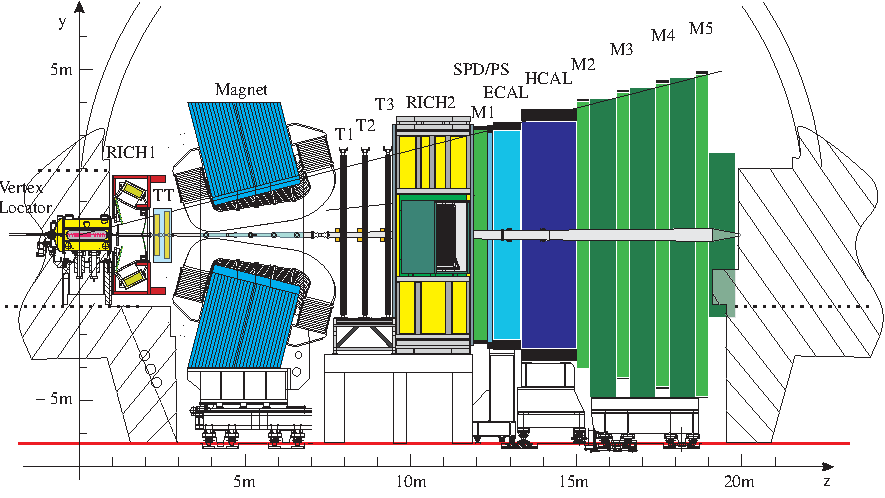
\includegraphics[width=0.7\textwidth]{figs/lhcb_detector_view.pdf}
    \caption{
        View of the LHCb detector and its subsystems.
        Extracted from \cite{LHCb:2003ab}.
    }
    \label{fig:lhcb_detector_view}
\end{figure}

% Talk about LHCb being forward-only
An interesting design choice is the geometry of the LHCb detector:
Instead of being a barrel $4\pi$ detector, it is forward-only.
This is because at high energies, $b\bar{b}$ is mostly produced in the forward
and backward direction.
The LHCb design is a very cost-effective way to construct a detector at the LHC
dedicated for $B$ physics.

% Talk about tracking
LHCb has a very good vertexing and tracking system, achieving vertex resolutions
down to 20~$\mu$m in a challenging environment.
However, due to the amount of material before the calorimeters and their poor
granularity,
reconstruction of neutral particles, such as $\pi_0$, is less
precise \cite{LHCb:2008,Guz:2017}.
This is why LHCb analyses typically focus on final states with charged particles
only, whereas $B$ factories can afford to use final states with neutral
particles.

% Talk about run 1 and run 2 luminosity
LHCb collected data from 2010 to 2012 with a center of mass energy of
\SI{8}{TeV}, and from 2015 to 2018 at \SI{13}{TeV}.
The total integrated luminosity during these two periods is about
\SI{9.2}{fb^{-1}} \cite{LHCb-Lumi:2019}.
% Talk about LS2 upgrade and LHCb's future
Currently, LHCb is shut down for an upgrade which will greatly increase the
readout rate of the detector starting in 2021.



\section{Review of previous measurements of \RDDst/}
In this section, I will review some of the more important results of LFU
measurements.
I will focus on \BaBar/ and LHCb results, but related measurement results from
other experiments, such as BELLE, will also be listed.


\subsection{2013 \BaBar/ \RDDst/}
This paper \cite{Lees:2013uzd} is the first measurement that observers an excess
in the \RD/ and \RDst/ ratio:
There is a $2.0 \sigma$ and $2.7 \sigma$ deviation from the SM, for \RD/ and
\RDst/ respectively, and a combined $3.4 \sigma$ deviation.
I will review some of the techniques applied in this analysis.

The signature of a semileptonic $B$ decay into $\tau$, such as
$B^0 \longrightarrow D^{-(*)} (\longrightarrow \text{various modes})
\tau^+ (\longrightarrow \mu^+ \nu_{\mu} \bar{\nu}_{\tau}) \nu_{\tau}$, is the
non-zero missing mass:
Since $\tau$ has a very short lifetime, it decays into a $\mu$ and two
neutrinos;
this results in a 3-neutrino final state.
Now, the missing mass $m_{miss}$ is defined to be:
\begin{equation*}
    m_{miss} \equiv \left(p_{B_{sig}} - p_{visible}\right)^2
\end{equation*}
if there is only one neutrino, then $m_{miss} = m_{\nu} \approx 0$;
on the other hand, three neutrinos very frequently gives non-zero $m_{miss}$.

Hence, it is crucial to find $p_{B_{sig}}$.
In a $e^- e^+$, collider, the invariant mass is known.
As long as we find the momentum of the other $B$ meson, denoted as
$p_{B_{tag}}$, we know $p_{B_{sig}}$;
that is, we tag the decay of the \Y4S/:
\begin{equation*}
    \Y4S/ \longrightarrow B \overline{B} \xrightarrow{\text{tagging}}
        B_{tag} B_{sig}
\end{equation*}

\BaBar/ and BELLE independently developed two types of tagging algorithms:
semileptonic tagging and hadronic tagging.
Semileptonic tagging finds $B_{tag}$ with the following decay:
$B^+ \longrightarrow l^+ \nu_l$, where $l+$ is $e^+ or \mu^+$.
This has the advantage of a larger branching ratio, thus more ($\approx 1\%$)
\Y4S/ events are tagged.
However, in this type of events, at least two neutrinos are presents, which
makes the reconstruction of $p_{B_{sig}}$ less precise \cite{Ciezarek:2017yzh}.

In this paper, hadronic tagging algorithm is improved and used:
It listed a very large number of hadronic decay chains of $B$;
for each \Y4S/ event, it compares the decay product of each $B$, tagging the
ones that match one of the listed modes.
This has a smaller tagging rate ($\approx 0.3$), but because the tagging side
momentum is reconstructed precisely (no neutrino, so all hadronic particles are
in principle reconstructed), the estimation on $p_{B_{sig}}$ is better, which
leads to a more precise measurement on
$m_{miss}$ \cite{Lees:2013uzd,Ciezarek:2017yzh}.

Another interesting technique is the usage of Gaussian non-parametric kernel
estimators in the fit.
This method has the added benefit of knowing the exact relation between variance
and bias, making optimization easier.
After numerous validation processes, it is concluded that the kernel estimators
performed well \cite{Lees:2013uzd}.

% BELLE measurements
BELLE experiment at KEK measured semileptonic $B$ decays with $\tau$ decay both
leptonically and hadronically.
Both semileptonic and hadronic tagging were used for the leptonic $\tau$ decay;
for hadronic $\tau$ decay, only hadronic tag was used.
The overall \RDDst/ deviation from the SM is about
$2\sigma$ \cite{Hirose:2017185}.

\subsection{2015 LHCb \RDst/}
The 2015 LHCb \RDst/ paper reports
$\RDst = 0.336 \pm 0.027 \text{(stat)} \pm 0.030 \text{(syst)}$, which is
$2.1 \sigma$ larger than the SM prediction \cite{LHCb:PhysRevLett.115.111803}.

One interesting choice of this analysis is that it concerns only one
semileptonic decay mode:
$\overline{B}^0 \longrightarrow D^{*+} l^- \overline{\nu}_l$.
Because all the final products, except for $\overline{\nu}_l$, are charged,
making reconstruction easier for LHCb \cite{LHCb:PhysRevLett.115.111803}.

Since the center of mass energy is unknown in hadron colliders, previous tagging
algorithms for $e^- e^+$ detectors cannot be used.
To estimate $p_{B}$, a new rest frame approximation method is developed:
Assuming $\vec{(p_{B})_T}$ is unchanged, approximate $(p_{B})_z$ by the
following:
\begin{equation*}
    (p_{B})_z = \frac{m_B}{m_{reco}} (p_{reco})_z
\end{equation*}
with $m_B$ the known $B$ mass.
This is shown to have sufficient resolution \cite{LHCb:PhysRevLett.115.111803}.


% 2018 LHCb hadronic decay of Tau -> 3* Pi R(D*)

\section{Outlook for LHCb Run 2 \RDDst/ measurements}
% Expected improvements
% Remember: Run 2 supposedly has better pile-ups.

% Current progress


\PRLrule
\printbibliography
\end{document}
